\documentclass{article} % For LaTeX2e
\usepackage{nips13submit_e,times}
\usepackage{hyperref}
\usepackage{url}
\usepackage{listings}
\usepackage{amsmath}
\usepackage{graphicx}
\usepackage{xcolor,colortbl}
\usepackage{slashbox}
\usepackage{hhline}
\usepackage{float}
\restylefloat{table}

    \renewcommand{\topfraction}{0.9}	% max fraction of floats at top
    \renewcommand{\bottomfraction}{0.8}	% max fraction of floats at bottom
    %   Parameters for TEXT pages (not float pages):
    \setcounter{topnumber}{2}
    \setcounter{bottomnumber}{2}
    \setcounter{totalnumber}{4}     % 2 may work better
    \setcounter{dbltopnumber}{2}    % for 2-column pages
    \renewcommand{\dbltopfraction}{0.9}	% fit big float above 2-col. text
    \renewcommand{\textfraction}{0.07}	% allow minimal text w. figs
    %   Parameters for FLOAT pages (not text pages):
    \renewcommand{\floatpagefraction}{0.7}	% require fuller float pages
	% N.B.: floatpagefraction MUST be less than topfraction !!
    \renewcommand{\dblfloatpagefraction}{0.7}	% require fuller float pages

\title{Predicting Starcraft 2 Player Skill}
\author{Forrest Coward}

\newcommand{\fix}{\marginpar{FIX}}
\newcommand{\new}{\marginpar{NEW}}
\nipsfinalcopy % Uncomment for camera-ready version

\begin{document}
\maketitle

\begin{abstract}
Starcraft II is popular a real time strategy game developed by Blizzard Entertainment. In its primary game mode, two players compete against one another in an online match of strategic and tactical dominance. Players are placed into one of seven possible leagues depending on their skill level. Given a replay file of a Starcraft II match, the goal of this paper is to predict the  league of its players using decision trees and random forests. 
\end{abstract}

\section{Overview of Starcraft 2}

This section provides brief background information regarding Starcraft II. 
\subsection{Leagues}

In order to differentiate between the skill of different players, each player is placed into a league based on their performance over many games. There are seven different leagues, each which contain a percent of the active player base. From worst to best the leagues are: bronze (8\%), silver (20\%), gold (32\%), platinum (20\%), diamond (18\%), master (2\%), grandmaster (top 200 players). League placement is not fixed. With good performance, a player may be promoted to a higher league. Likewise, continual poor play may warrant a demotion. 

\subsection{Replays}

Every Starcraft  game produces replay file that exactly specifies the events of a particular game. Example events are a player moving his camera, a player selecting a hotkey, a unit being created, chat messages sent etc. Replays also contain metadata information such as game length and player names. Replays are useful for analyzing strategy, sharing exciting games with others, and most importantly, data analysis. 

\section{Task: League Prediction}

Given a Starcraft 2 replay file, we want to predict the league of one or both of its players. 

More specifically, each replay produces two data points: one for each player (that is, given the events in the replay file that pertain to a particular player, predict the league of said player). There are two steps involved to make this possible. First, features for each player must be extracted from the replay to form the data set. Second, machine learning algorithms must be applied to the data set to predict the league of the player. 

\section{Extracting Data From Replay Files}

This section explains how replay files were gathered and parsed. 

\subsection{Parsing Replays - SC2Reader}

SC2Reader\footnote{\url{https://github.com/GraylinKim/sc2reader}} is Python library for parsing Starcraft 2 replay files. It abstracts away the low level details of the file format making it easy to extract game state. Example usage is shown below:

\

\lstset{frame=shadowbox, rulesepcolor=\color{white}}
\lstset{language=Python} 
\begin{lstlisting}
replay = sc2reader.parse_replay(replay_file)
players = replay.players
for event in replay.game_events:
	// process event
\end{lstlisting}

\subsection{Retrieving League Information}

A replay file does not include the leagues of the players at the time the game was played. Instead, a player's current league (as well as their highest league ever acheived) is viewable on their unique Battle.net profile page managed by Blizzard. Unfortunately, Blizzard does not expose an \emph{API} to query for this data. To circumvent this problem, I wrote a web scrapper that given a player's profile \emph{URL}, returns the league history of the player.

\subsection{Gathering Replays}

Blizzard recently updated the replay file format to version \emph{2.0.8.25604}. This new format includes a plethora of additional metadata to aid in statistical analysis \footnote{\url{http://us.battle.net/sc2/en/blog/9669862/StarCraft_II_Patch_208_Replay_File_Enhancements-5_7_2013}}. Part of this metadata is a polling of certain parts of the game state every ten seconds. This makes it easy to directly compute statistics such as average unspent resources, which was notoriously difficult to determine correctly prior to this update. 

Thus, using the latest replay format is practically a requirement for extracting good features from the replays. However, due to the limited time this format has been in use, the vast majority of Starcraft 2 replays on the web cannot be used for this paper. 

 
Luckily, \url{http://drop.sc}, the most popular Starcraft 2 replay uploading website, adds more than two-hundred \emph{2.0.8.25604} replays a day. Due to a lack of a bulk download option, I wrote a script to crawl \url{drop.sc} and download relevant replays to disk.

\section {Data Set}

Each replay produces two data points: one for each player. The final data set consists of \(135\) data points from each league for a total of \(945\) data points.

\section{Feature Selection} 

This section overviews the feature selection process. 

\subsection{Feature Selection Commentary}

In Starcraft 2, players choose to play as one of three races: Terran, Protoss or Zerg. Each race has their own set of structures, units and production cycles. For example, Terran may only build one unit at a time from each production structure, but may queue up to five units simultaneously. On the other hand, Zerg morph all their units from larva, which regularly spawn around a Hatchery. The existence of different units and structures makes it difficult to create features common to all races. Ideal features can identify player skill despite the race they play.

One possibility is to classify units into tiers. Tier 1 units have relatively few prerequisites and thus are always used in the early game. Tier 3 units have more requirements and are generally more expensive, and thus are only seen in the late game. We could hypothesize that better players use higher tier units on average, however, the tier of a unit is not correlated with its effectiveness. For example, it is common for Terran players to rely on mass tier 1 and 2 units.  Another possibility is to count the number of skill units built. Skill units require extensive amount of control and attention from the player to be effective, thus, we would expect higher skilled players to utilize these units more on average. Unfortunately, this is likely not a great metric. Skill units are too situational depending on the game and matchup. In the end, I decided not to use features involving specific racial units, despite writing code to query this information from a replay. 

There are many game mechanics similiar among the races such as worker units, resource collection and supply limits. Each race has a unique worker unit that collects the two types available resources: minerals and vespene gas. The amount of workers required and resource collection rates these provide are roughly the same for all three races, making these statistics useful feature constructors. 

Game duration is another factor that must be considered in relation to certain features. For example, in shorter games, we expect lower resource collections rates and less time spent supply blocked. As the game goes on, an optimal amount of workers are created and resource collection rates reach a maximum. The amount of time a player spends supply blocked will increase as multitasking skills are stressed. In a very long game, resources become more scarce as fight to secure the remaining resources on the map. I do not concern myself with game duration under the assumption there will be nice averages with a large number of replays. However, I did throw out games lasting under eight minutes. In the first few minutes of the game, there is little a great player can do to differentiate themselves from a lesser foe.

Finally, there are features of the player's actions. The most notable is the actions per minute (\emph{APM}) metric that measures multitasking ability. Other features in this category include number of hotkeys used and number of times  a player issues a command to the minimap.

\subsection{Selected Features}

Below is a table of the selected features and their possible values:

	\renewcommand{\arraystretch}{1.25}
	\begin{tabular}{ | l | l | l |   p { 5cm}}
	\hline {\bf Feature} & {\bf Explanation} & {\bf Value} \\
	\hline League & the league the player & \({ 1, 2, 3, 4, 5, 6, 7 }\) \\
	\hline APM & actions completed per minute & float \\
	\hline Hotkeys & number of hotkeys used  & low (1-3), medium (4- 6), high (7-9) \\
	\hline Minimap & number of times minimap is clicked & int \\
	\hline Mineral Collection Rate & average minerals collected per minute & float \\
	\hline Vespene Collection Rate & average vespene gas collected per minute & float \\
	\hline Average Unspent Minerals & average unspent minerals per minute & float \\
	\hline Average Unspent Vespene & average unspent vespene gas per minute & float \\
	\hline Spending Quotient & \(35*(0.00137*C - log(U)) + 240\)  & float \\
	\hline Worker Rate  & workers built per minute & float \\
	\hline Supply & \% of game duration spent supply capped & float 0-100  \\
	\hline Unique Units & number of unique units created & int\\
	\hline Mannered & 1 if player sends '\emph{gg}' or '\emph{gg wp}'  message & \({ 0, 1}\) \\
	\hline
	\end{tabular}

Note: in the spending quotient equation, \emph{C} is the average resource collection rate and \emph{U} is the average unspent resources \footnote{\url{http://wiki.teamliquid.net/starcraft2/Spending_quotient}}.

\vspace{2 mm}

Table 1 (see below) displays the average value of each feature across each league. Overall, features trend quite nicely across.  The clear exception to this is the mannered feature which does not appear to be correlated with league. One interesting point is that MCR and VCR actually slightly decrease from master to grandmaster, however, spending quotient still increases. This means that while master and grandmaster players collect on average the same amount of resources, grandmasters spend the resources more efficiently. This is also reflected in the decrease of AUM and AUV from master to grandmaster. 

\begin{table}[H]
\renewcommand{\arraystretch}{1.25}
\label{tab:average_values}
\caption {Average value of selected features for each league} 
\vspace{3 mm}
    \begin{tabular}{|c|ccccccc|}
    \hline
                    & \textbf{Bronze} & \textbf{Silver} & \textbf{Gold} & \textbf{Platinum} & \textbf{Diamond} & \textbf{Master} & \textbf{GM} \\ \hline
    \textbf{APM}          & 42.7   & 53.8   & 70.8 & 77.3     & 103.7   & 128.2  & 156.8       \\ \hline
    \textbf{Hotkeys}      & 1.9    & 2.6    & 3.2  & 3.3      & 3.9     & 4.9    & 5.6         \\ \hline
    \textbf{Minimap}      & 14.8   & 29.8   & 33.5 & 37.8     & 49.5    & 59.6   & 66.7        \\ \hline
    \textbf{MCR}          & 719    & 823    & 902  & 931      & 993     & 1033   & 1030        \\ \hline
    \textbf{VCR}          & 209    & 223    & 253  & 258      & 282     & 294    & 289         \\ \hline
    \textbf{UM}           & 1074   & 902    & 860  & 730      & 653     & 540    & 412         \\ \hline
    \textbf{UV}           & 515    & 461    & 445  & 415      & 388     & 370    & 313         \\ \hline
    \textbf{SQ}           & 35.6   & 46.1   & 53.6 & 58.7     & 66.2    & 73.8   & 81.3        \\ \hline
    \textbf{Worker Rate}      & 2.12   & 2.64   & 2.81 & 3.15     & 3.46    & 3.62   & 3.75        \\ \hline
    \textbf{Supply}       & 8.30   & 8.08   & 8.50 & 7.76     & 7.82    & 7.43   & 6.77        \\ \hline
    \textbf{Unique Units} & 6.54   & 6.55   & 6.92 & 7.14     & 7.46    & 7.68   & 7.72        \\ \hline
    \textbf{Mannered}     & .10    & .14    & .18  & .17      & .15     & .15    & .14         \\ \hline
    \end{tabular}
\end{table}

\section{Data Analysis with Decision Trees and Random Forests}

Decision trees and random forests are the primary machine learning tools used in this paper. 

\subsection {Decision Tree Algorithm}

The decision tree induction algorithm is rather simple and will not be covered in detail. However, there are a few specifics that are important to point out regarding how each tree is constructed: 

\begin{itemize}
\item 
Each decision tree node performs one split (except for leafs)
\item
When splitting on continous attributes, the continous range for that attribute is discretized because an exhaustive search of every value for the optimal split would take too long. For example, if there was some attribute with a large number of continous values between [0, 1000] the algorithm would examine the strength of splitting at 200, 400, 600, 800 (in addition to examining the strength of split of other attributes). 
\item
Post pruning is performed to merge leaves of the same majority class

\end{itemize}

\subsection{Decision Tree Split Metrics}

The best split for a decision tree node is one that produces the most pure children nodes (i.e. increases the certainty of our prediction). Let \(p(i | n)\) be the fraction of records belonging to class \(i\) at a given node \(n\). Let \(c\) be the number of classes. We can now define several different split metrics.

\begin{itemize}
\item
Information Gain: the expected decreased in entropy

 \(entropy(n) = -\sum_{i=0}^{c-1} p(i|n)\log _2 \left( p(i|n) \right)\)
\item
Gini Index: the probability that two randomly chosen data points will have different classes

 \(gini(n)=1-sum_{i=0}^{c-1} [p(i|n)]^2 \)
\item
Gain Ratio: information gain divided by the entropy of an attribute's possible values. The forumla is slightly more complex and is omitted. Inuitively, gain ratio biases the decision tree against considering attributes with a large number of distinct values, which is a problem with both information gain and the gini index. 

\end{itemize}

\subsection{Experiment: Varying Tree Depth and Split Metrics for Standard Decision Trees}

Figure 1 illustrates the classification accuracy of standard decision trees varying the split metric used and the depth of tree. The best accuracy is acheived using the gini index on a tree of depth seven. Also observe that  gini index performs better than information gain and gain ratio for most depths. Accuracy ceases to increase starting around depth six, suggesting the amount of useful features is limited to around six or seven (since the same attribute is not generally split twice down the same path). Gain ratio performing worse than the other metrics makes sense: many continuous features discretize into a large number of discrete values, for which information gain and gini index are biased. 

\setlength{\abovecaptionskip}{-20pt}
\begin{figure}
\vspace*{-.5in}
\hspace*{-.9in}
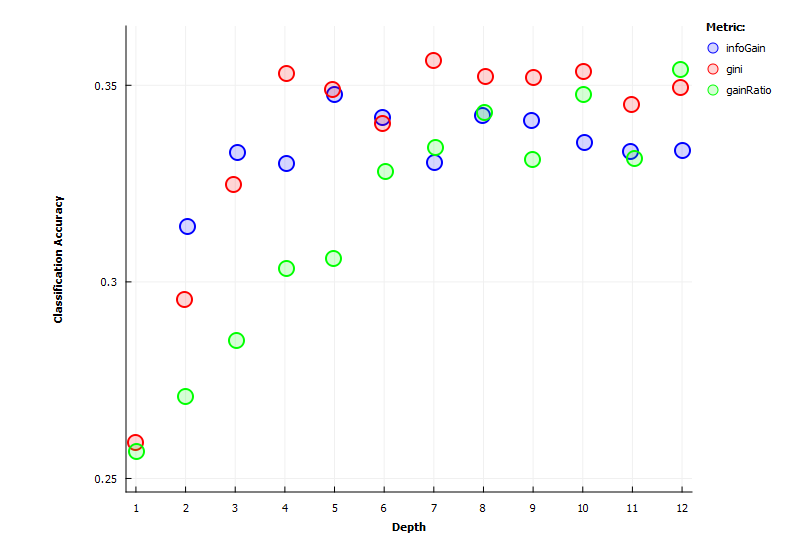
\includegraphics[width=174mm]{decision_trees.png}
\caption{classification accuracy versus depth of the decision tree for different split metrics (5-fold cross validation)}
\end{figure}


\subsection{Experiment: Varying Number of Trees and Number of Randomly Selected Features  in Random Forest}

Random forest is an ensemble classifcation method. It works by creating many decision trees using a random subset of the features for each tree and outputting the class that is the mode of the classes selected by the indivdual trees. 

Figure 2 illustrates the classification accuracy of random forests by varying the number of trees in the forest and the number of randomly selected attributes used per tree. There are a few useful observations. First, classification accuracy using random forests is quite a bit better than using an individual decision tree. Second, classification accuracy stops increasing when using more than five randomly selected features. Again, this suggests many features are not useful. Third, using around one-hundred trees for this problem appears to be ideal. In general, the number of trees required is a function of the total number of features and the number of random features used to construct each tree. Imagine using a very large number of features, two random features per tree, and only having five trees in the forest. Clearly, these five trees are insufficient to capture all pairs of feature combinations. 

\begin{figure}
\vspace*{-.5in}
\hspace*{-.6in}
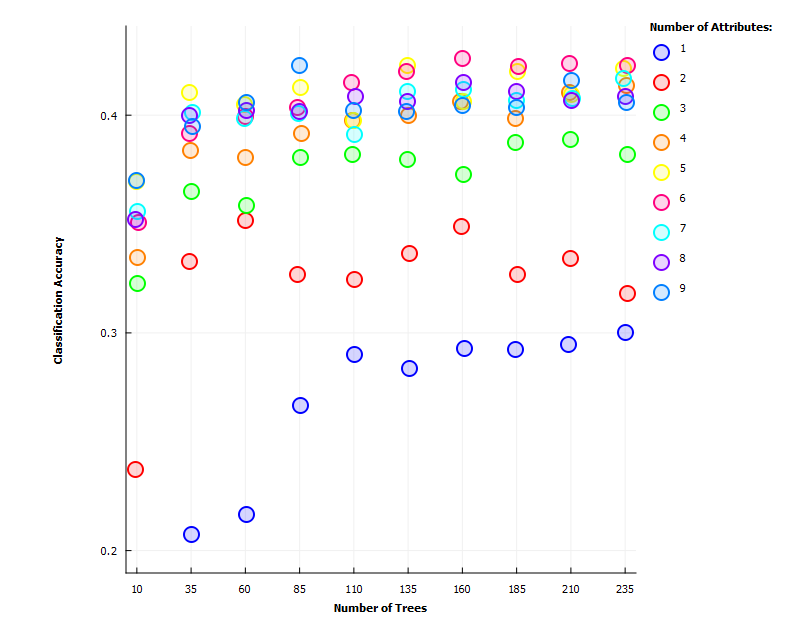
\includegraphics[width=174mm]{random_forests.png}
\caption{classification accuracy versus number of trees for different number of randomly selected attributes per tree (5-fold cross validation) }
\end{figure}

\subsection{Experiment: Feature Selection Using Random Forests}

Random forests can be used more formally for feature selection. The basic idea is that for an important feature, classlification accuracy decreases when that feature is left out of a tree. Over many trees, we can rank which features give the best classification results. To create the ranking, we just compare the errors between all trees with the feature included versus the trees with it excluded. Below is the ranking for the top six features (to save space). The unshown remaining rankings are [hotkeys: \(.50\)], [workers, .\(49\)], [AUV, \(.41\)], [supply, \(.14\)], [unique, \(.01\)], [mannered, \(-.07\)]. 


\begin{center}
\begin{table}[H]
    \begin{tabular}{|l|c|}
    \hline
    \textbf{Feature}  &\textbf{Score} \\ \hline
    APM      & 7.36  \\ \hline
    SQ       & 5.30  \\ \hline
    Minimap  & .75   \\ \hline
    AUM      & .74   \\ \hline
    MCR      & .60   \\ \hline
    VCR      & .51   \\ \hline
    \end{tabular}
\end{table}
\end{center}

These results show that two features, APM and SQ (spending quotient), are by far the best predictors of league. The next four to five features are helpful, but not by that much. Indeed, figure 2 illustrates that combinations of five or six features is just as good as a combination of eight or nine (or more). Similarly, any accuracy gains quickly dimish past two features. 

  



\section{Overall Results} 

Table 2 displays classification rates for a number of different supervised learning algorithms. The within one league accuracy is the amount of data points correctly classified within an error of one league. 

\setlength{\abovecaptionskip}{+7pt}
\begin{table}[H]
\caption {Classification accuracies for different supervised learning algorithms (5-fold cross validation)  } 
    \begin{tabular}{| c | c | c |}
    \hline
    \textbf{Method}             & \textbf{Classification Accuracy} & \textbf{Within One League Accuracy} \\ \hline
    Best Random Forest  & \textbf{42.43\%}                  & 74.28\%            \\ \hline
    Naive Bayes         & 37.25\%                  & 71.74\%            \\ \hline
    Linear SVM          & 37.57\%                  & \textbf{78.09\%}            \\ \hline
    Best Decision Tree  & 35.87\%                  & 70.88\%            \\ \hline
    10-Nearest-Neighbor & 29.31\%                  & 64.97\%            \\ \hline
    \end{tabular}
\end{table}

Random forests had by far best classification accuracy, however, a simple linear support vector machine had a better within one league classification accuracy. How could this be? Here is a hypothesis: decision trees try to optimize their classification accuracy without explicit knowledge of the distribution of classes (or relationship between classes, such as bronze leauge being very similar to silver league). This works better when classes are very distinct, such as 'Yes' or 'No'. On the other hand, support vector machines are defined by the distribution (the layout of data points in space) and allow for some amount of tolerance for misclassified points within a boundary. So while a support vector machine may do worse for straight up classification, it has a better feel for the total distribution of data points, and thus does better when there is an error of one league. More analysis is required on this topic, but is outside the scope of this paper. 

\subsection{Explaining the Low Correct Classification Rate}

At first glance the results from table 2 appear pretty poor. The best algorithm was random forests with a correct classifcation rate of \(42.5\%\). This is large improvement from a random guess (one out of seven), but still not particularly great considering the average trends in the features across leagues are well defined (see table 1).

Table 3 is a confusion matrix for a sample classification distribution. Note that the classification distribution for different methods all are similar in shape to this.
\setlength{\abovecaptionskip}{+13pt}
\begin{table}[H]
\renewcommand{\arraystretch}{1.3}
\caption {Confusion matrix for a thirty tree random forest using five randomly selected attributes per tree (5-fold cross validation). Correct class is on the left while prediction is on the top.  } 
\vspace{2 mm}
    \begin{tabular}{@{}| c | c  c  c  c  c  c  c | c  c  c  | @{}}
   \hline
    League   &1   & 2   & 3  & 4   & 5   & 6   & 7   & Total & Correct & Within One \\ \hline
    1     &  \cellcolor{green}85  &  \cellcolor{green!25}29  & 14 & 4   & 3   & 0   & 0   & 135 & .623 &  .844 \\ 
    2     & \cellcolor{green!25} 39  &  \cellcolor{green}48  &  \cellcolor{green!25}26 & 9  & 7   & 4   & 2   & 135 & .355 & .837  \\ 
    3     & 17  &  \cellcolor{green!25}30  &  \cellcolor{green}48 &  \cellcolor{green!25}17  & 15  & 6   & 2   & 135  & .355 & .704 \\
    4     & 9  & 26  &  \cellcolor{green!25}33 &  \cellcolor{green}22  &  \cellcolor{green!25}22  & 16  & 7  & 135 & .163 & .570  \\
    5     & 2   & 10  &18 &  \cellcolor{green!25}16  &  \cellcolor{green}47  &  \cellcolor{green!25}24  & 18  & 135 & .348 & .644  \\
    6     & 2   & 1   & 10  & 6   &  \cellcolor{green!25}19  &  \cellcolor{green}63  &  \cellcolor{green!25}34  & 135  & .466 & .859 \\
    7     & 1   & 0   & 3  & 6   &24  & \cellcolor{green!25} 32  &  \cellcolor{green}69  & 135  & .511 & .748  \\\hline
    Total & 155 & 144 & 152 & 80 & 137 & 145 & 132 & 945 & \cellcolor{green}.404 &\cellcolor{green!25} .744 \\
   \hline
    \end{tabular}
\end{table}

A key thing to note here is that the classification of leagues one, six, and seven are the most accurate. These leagues represent a very small minority of the player base on each side of the spectrum (bronze is the bottom \(8\%\) of the players, while master and grandmasters are the top \(~2\%\)) and stand out statistically. Correct classification rates are especially poor for the middle leagues. In table 3, only \(16.3\%\) of those in league four were correcly classified as such. The overall low classification accuracy suggest that there is a lot of noise in the data set and that many similar data points have different leagues (the results for 10-nearest-neighbor are especially indicative). 

\subsection{The Problem Of Modeling League as a Discrete Value}

Modeling player skill as a discrete value is problematic. In reality, each player has a hidden match making rating (MMR) that represents a point on the  continous distribution of skill. Leagues are a method of discretizing MMR to make ranking simpler to the player. 

Furthermore, MMR distribution overlaps between leagues. This means there are a number of players in each league that have an MMR that falls inside the MMR distribution of another league. This phenomona has greater effect on the central leagues, as there will be overlap on each side of the distribution (thus causing worse classification). 

Another problem is players may not always have an MMR (or league) that represents their true skill. For example, a grandmaster level player who starts a new account begins with a low MMR. It will take a large number of wins before their MMR approaches their true skill and they are placed as a grandmaster. This is problematic for this paper because it means the league of a player may have no correlation with their skill. Unfortunately, there is no way to detect the stabalization of a player's MMR (or even the MMR itself). A possible solution is to not count a data point if the particular player representing that data point has played less than some amount of games. 

\subsection{A Better Classification Error: Within One League}

For the reasons stated above, the within one league classification accuracy was introduced. Again, this is simply the percent of data points classified correctly within an error of one league. Observe in table 3 that bronze league player is never misclassified as grandmaster, but is often misclassfied as silver and sometimes misclassified as gold. Likewise, only in a single case is grandmaster misclassified as bronze. This means that despite many classifications being incorrect, these supervised learning methods are often close to the correct answer. Thus, this metric better captures the overlap between MMR distributions. Indeed, the classification accuracy almost doubles if we allow an error of one league.

\section{Summary}

Random forests are three times more likely to correctly predict the league of a player than chance and vastly out perform standard decision trees. If allowed an error of one league, random forests have \(75\%\) accuracy and are roughly twice as good as chance. Random forest parameter experimentation and feature scoring revealed similar results could be acheived by just using the top five to six features, though two features in particular were much better than the rest: actions per minute and spending quotient. Other supervised learning methods performed similarly to standard decision trees but were not as effective as random forests for exact classification accuracy. 

\section{Future Work}

Possible future work includes:

\begin{itemize}
\item
Use regression instead of classification to better model the true skill of each player
\item
Take into account the prior distribution of leagues
\item
Perform race by race analysis (richer features per race)
\item
Experiment with unsupervised learning methods
\end{itemize}

\section{References}

\small{
[1] Breiman, Leo (2001) \emph{Random Forests}, http://link.springer.com/content/pdf/10.1023%2FA%3A1010933404324.pdf

[2] \emph{Classification: Basic Concepts, Decision Trees, and Model Evaluation}, http://www-users.cs.umn.edu/~kumar/dmbook/ch4.pdf

[3] \emph{Analysis of macro across all teirs of the SC2 ladder}, http://www.teamliquid.net/forum/viewmessage.php?topic\_id=266019

[4] Blair, Mark (2013) \emph{Starcraft II + Science}, http://www.teamliquid.net/forum/viewmessage.php?topic\_id=401425

[5] \emph {Predicting the result of a StarCraft 2 game}, http://joi.degn.de/node/31
}

\end{document}